\PassOptionsToPackage{unicode=true}{hyperref} % options for packages loaded elsewhere
\PassOptionsToPackage{hyphens}{url}
\PassOptionsToPackage{dvipsnames,svgnames*,x11names*}{xcolor}
%
\documentclass[8pt,ignorenonframetext,dvipsnames]{beamer}
\usepackage{pgfpages}
\setbeamertemplate{caption}[numbered]
\setbeamertemplate{caption label separator}{: }
\setbeamercolor{caption name}{fg=normal text.fg}
\beamertemplatenavigationsymbolsempty
% Prevent slide breaks in the middle of a paragraph:
\widowpenalties 1 10000
\raggedbottom
\setbeamertemplate{part page}{
\centering
\begin{beamercolorbox}[sep=16pt,center]{part title}
  \usebeamerfont{part title}\insertpart\par
\end{beamercolorbox}
}
\setbeamertemplate{section page}{
\centering
\begin{beamercolorbox}[sep=12pt,center]{part title}
  \usebeamerfont{section title}\insertsection\par
\end{beamercolorbox}
}
\setbeamertemplate{subsection page}{
\centering
\begin{beamercolorbox}[sep=8pt,center]{part title}
  \usebeamerfont{subsection title}\insertsubsection\par
\end{beamercolorbox}
}
\AtBeginPart{
  \frame{\partpage}
}
\AtBeginSection{
  \ifbibliography
  \else
    \frame{\sectionpage}
  \fi
}
\AtBeginSubsection{
  \frame{\subsectionpage}
}
\usepackage{lmodern}
\usepackage{amssymb,amsmath}
\usepackage{ifxetex,ifluatex}
\usepackage{fixltx2e} % provides \textsubscript
\ifnum 0\ifxetex 1\fi\ifluatex 1\fi=0 % if pdftex
  \usepackage[T1]{fontenc}
  \usepackage[utf8]{inputenc}
  \usepackage{textcomp} % provides euro and other symbols
\else % if luatex or xelatex
  \usepackage{unicode-math}
  \defaultfontfeatures{Ligatures=TeX,Scale=MatchLowercase}
\fi
% use upquote if available, for straight quotes in verbatim environments
\IfFileExists{upquote.sty}{\usepackage{upquote}}{}
% use microtype if available
\IfFileExists{microtype.sty}{%
\usepackage[]{microtype}
\UseMicrotypeSet[protrusion]{basicmath} % disable protrusion for tt fonts
}{}
\IfFileExists{parskip.sty}{%
\usepackage{parskip}
}{% else
\setlength{\parindent}{0pt}
\setlength{\parskip}{6pt plus 2pt minus 1pt}
}
\usepackage{xcolor}
\usepackage{hyperref}
\hypersetup{
            pdftitle={Introduction to Multivariate Regression \& Program Evaluation},
            pdfauthor={Lecture 13},
            colorlinks=true,
            linkcolor=Maroon,
            filecolor=Maroon,
            citecolor=Blue,
            urlcolor=blue,
            breaklinks=true}
\urlstyle{same}  % don't use monospace font for urls
\newif\ifbibliography
\usepackage{graphicx,grffile}
\makeatletter
\def\maxwidth{\ifdim\Gin@nat@width>\linewidth\linewidth\else\Gin@nat@width\fi}
\def\maxheight{\ifdim\Gin@nat@height>\textheight\textheight\else\Gin@nat@height\fi}
\makeatother
% Scale images if necessary, so that they will not overflow the page
% margins by default, and it is still possible to overwrite the defaults
% using explicit options in \includegraphics[width, height, ...]{}
\setkeys{Gin}{width=\maxwidth,height=\maxheight,keepaspectratio}
\setlength{\emergencystretch}{3em}  % prevent overfull lines
\providecommand{\tightlist}{%
  \setlength{\itemsep}{0pt}\setlength{\parskip}{0pt}}
\setcounter{secnumdepth}{0}

% set default figure placement to htbp
\makeatletter
\def\fps@figure{htbp}
\makeatother


%packages
\usepackage{graphicx}
\usepackage{rotating}
\usepackage{hyperref}

\usepackage{tikz} % used for text highlighting, amongst others
\usepackage{comment}

%title slide stuff
%\institute{Department of Education}
%\title{Managing and Manipulating Data Using R}

%
\setbeamertemplate{navigation symbols}{} % get rid of navigation icons:
\setbeamertemplate{footline}[page number]

%\setbeamertemplate{frametitle}{\thesection \hspace{0.2cm} \insertframetitle}
\setbeamertemplate{section in toc}[sections numbered]
%\setbeamertemplate{subsection in toc}[subsections numbered]
\setbeamertemplate{subsection in toc}{%
  \leavevmode\leftskip=3.2em\color{gray}\rlap{\hskip-2em\inserttocsectionnumber.\inserttocsubsectionnumber}\inserttocsubsection\par
}

%define colors
%\definecolor{uva_orange}{RGB}{216,141,42} % UVa orange (Rotunda orange)
\definecolor{mygray}{rgb}{0.95, 0.95, 0.95} % for highlighted text
	% grey is equal parts red, green, blue. higher values >> lighter grey
	%\definecolor{lightgraybo}{rgb}{0.83, 0.83, 0.83}

% new commands

%highlight text with very light grey
\newcommand*{\hlg}[1]{%
	\tikz[baseline=(X.base)] \node[rectangle, fill=mygray] (X) {#1};%
}
%, inner sep=0.3mm
%highlight text with very light grey and use font associated with code
\newcommand*{\hlgc}[1]{\texttt{\hlg{#1}}}

%modifying back ticks to add grey background
\let\OldTexttt\texttt
\renewcommand{\texttt}[1]{\OldTexttt{\hlg{#1}}}


\begin{comment}

% Font
\usepackage[defaultfam,light,tabular,lining]{montserrat}
\usepackage[T1]{fontenc}
\renewcommand*\oldstylenums[1]{{\fontfamily{Montserrat-TOsF}\selectfont #1}}

% Change color of boldface text to darkgray
\renewcommand{\textbf}[1]{{\color{darkgray}\bfseries\fontfamily{Montserrat-TOsF}#1}}

% Bullet points
\setbeamertemplate{itemize item}{\color{BlueViolet}$\circ$}
\setbeamertemplate{itemize subitem}{\color{BrickRed}$\triangleright$}
\setbeamertemplate{itemize subsubitem}{$-$}

% Reduce space before lists
%\addtobeamertemplate{itemize/enumerate body begin}{}{\vspace*{-8pt}}

\let\olditem\item
\renewcommand{\item}{%
  \olditem\vspace{4pt}
}

% decreasing space before and after level-2 bullet block
%\addtobeamertemplate{itemize/enumerate subbody begin}{}{\vspace*{-3pt}}
%\addtobeamertemplate{itemize/enumerate subbody end}{}{\vspace*{-3pt}}

% decreasing space before and after level-3 bullet block
%\addtobeamertemplate{itemize/enumerate subsubbody begin}{}{\vspace*{-2pt}}
%\addtobeamertemplate{itemize/enumerate subsubbody end}{}{\vspace*{-2pt}}

%Section numbering
\setbeamertemplate{section page}{%
    \begingroup
        \begin{beamercolorbox}[sep=10pt,center,rounded=true,shadow=true]{section title}
        \usebeamerfont{section title}\thesection~\insertsection\par
        \end{beamercolorbox}
    \endgroup
}

\setbeamertemplate{subsection page}{%
    \begingroup
        \begin{beamercolorbox}[sep=6pt,center,rounded=true,shadow=true]{subsection title}
        \usebeamerfont{subsection title}\thesection.\thesubsection~\insertsubsection\par
        \end{beamercolorbox}
    \endgroup
}

\end{comment}

\title{Introduction to Multivariate Regression \& Program Evaluation}
\providecommand{\subtitle}[1]{}
\subtitle{HED 612}
\author{Lecture 13}
\date{}

\begin{document}
\frame{\titlepage}

\begin{frame}
\tableofcontents[hideallsubsections]
\end{frame}
\begin{frame}{Where are we going\ldots{}.}
\protect\hypertarget{where-are-we-going.}{}

We have 3 lectures left!

\begin{itemize}
\tightlist
\item
  This Lecture {[}4/16/2020{]}

  \begin{itemize}
  \tightlist
  \item
    Non-linear functions cont.

    \begin{itemize}
    \tightlist
    \item
      Logs
    \end{itemize}
  \item
    Linear Probability Model

    \begin{itemize}
    \tightlist
    \item
      Using a 0/1 dummy dependent vairable
    \end{itemize}
  \item
    Reading:

    \begin{itemize}
    \tightlist
    \item
      Klasik, D., Blagg, K., \& Pekor, Z. (2018). Out of the Education
      Desert: How Limited Local College Options are Associated with
      Inequity in Postsecondary Opportunities. Social Sciences, 7(9),
      2018.
    \end{itemize}
  \item
    Homework Assignment \#13 will be posted soon!
  \end{itemize}
\end{itemize}

\medskip

\begin{itemize}
\tightlist
\item
  Next Lecture {[}4/23/2020{]}

  \begin{itemize}
  \tightlist
  \item
    Intro to interactions

    \begin{itemize}
    \tightlist
    \item
      Continuous by Categorical interactions
    \end{itemize}
  \item
    Review Klasik et al (2018)
  \end{itemize}
\end{itemize}

\medskip

\begin{itemize}
\tightlist
\item
  Next Next Lecture {[}4/30/2020, originally canceled on syllabus{]}

  \begin{itemize}
  \tightlist
  \item
    Categorical by Categorical interactions
  \item
    Continuous by Continuous interactions
  \end{itemize}
\end{itemize}

\medskip

\begin{itemize}
\tightlist
\item
  Reading Day, ``No Class'' {[}5/7/2020{]}
\end{itemize}

\end{frame}

\begin{frame}[fragile]{New R Package and Data!}
\protect\hypertarget{new-r-package-and-data}{}

We're going to try out a textbook I'm considering for HED 613 that comes
with an accopanying R package

\begin{itemize}
\tightlist
\item
  Applied Econometrics with R, Christian Kleiber \& Achim Zeileis
\item
  \href{https://rdrr.io/cran/AER/f/inst/doc/AER.pdf}{\texttt{AER}
  Package}

  \begin{itemize}
  \tightlist
  \item
    Comes with different functions and datasets!
  \end{itemize}
\end{itemize}

\medskip

Federal Reserve Bank of Boston under Home Mortgage Disclosure Act (HDMA)

\begin{itemize}
\tightlist
\item
  \texttt{HDMA} is a sample of mortgage applications filed in Boston in
  the 1990s
\end{itemize}

\end{frame}

\hypertarget{non-linear-functions-continued-logarithms}{%
\section{Non-linear functions Continued:
Logarithms}\label{non-linear-functions-continued-logarithms}}

\begin{frame}{Linear vs Non-Linear Models}
\protect\hypertarget{linear-vs-non-linear-models}{}

Two ways to think of ``non-linearity'':\ldots{}

\begin{itemize}
\tightlist
\item
  \textbf{Regression model that is a nonlinear function of the
  independent variables \(X_{1i}, X_{2i}... X_{ki}\)}

  \begin{itemize}
  \tightlist
  \item
    \_This can be estimated by OLS regression model via:

    \begin{itemize}
    \tightlist
    \item
      Polynomials
    \item
      Logarithms
    \item
      Interactions
    \end{itemize}
  \end{itemize}
\end{itemize}

\medskip

\begin{itemize}
\tightlist
\item
  Regression model that is a nonlinear function of the coefficients
  \(\beta_1, \beta_2... \beta_k\)

  \begin{itemize}
  \tightlist
  \item
    This can't be estimated by OLS!
  \item
    Only exception is \textbf{linear probability model}
  \end{itemize}
\end{itemize}

\end{frame}

\begin{frame}{Nonlinear functions of the IVs,
\(X_{1i}, X_{2i}... X_{ki}\)}
\protect\hypertarget{nonlinear-functions-of-the-ivs-x_1i-x_2i...-x_ki}{}

\begin{itemize}
\tightlist
\item
  OLS linear regression can model nonlinear function of the independent
  variables \(X_{1i}, X_{2i}... X_{ki}\) in two different ways!
\item
  \textbf{1. The effect of \(X_{1i}\) on Y depends on \(X_{1i}\)}

  \begin{itemize}
  \tightlist
  \item
    Ex: The negative effect of increasaing class size (x) on student
    test scores (Y) is ``bigger'' when initial class size is small
  \item
    Solution: polynomials and logged versions of X
  \end{itemize}
\item
  \textbf{2. The effect of \(X_{1i}\) on Y depends on \(X_{2i}\)}

  \begin{itemize}
  \tightlist
  \item
    Ex: The effect of class size (x) on student test scores (Y) depends
    on the teachers' years of experience
  \item
    Solution: interaction effects
  \end{itemize}
\end{itemize}

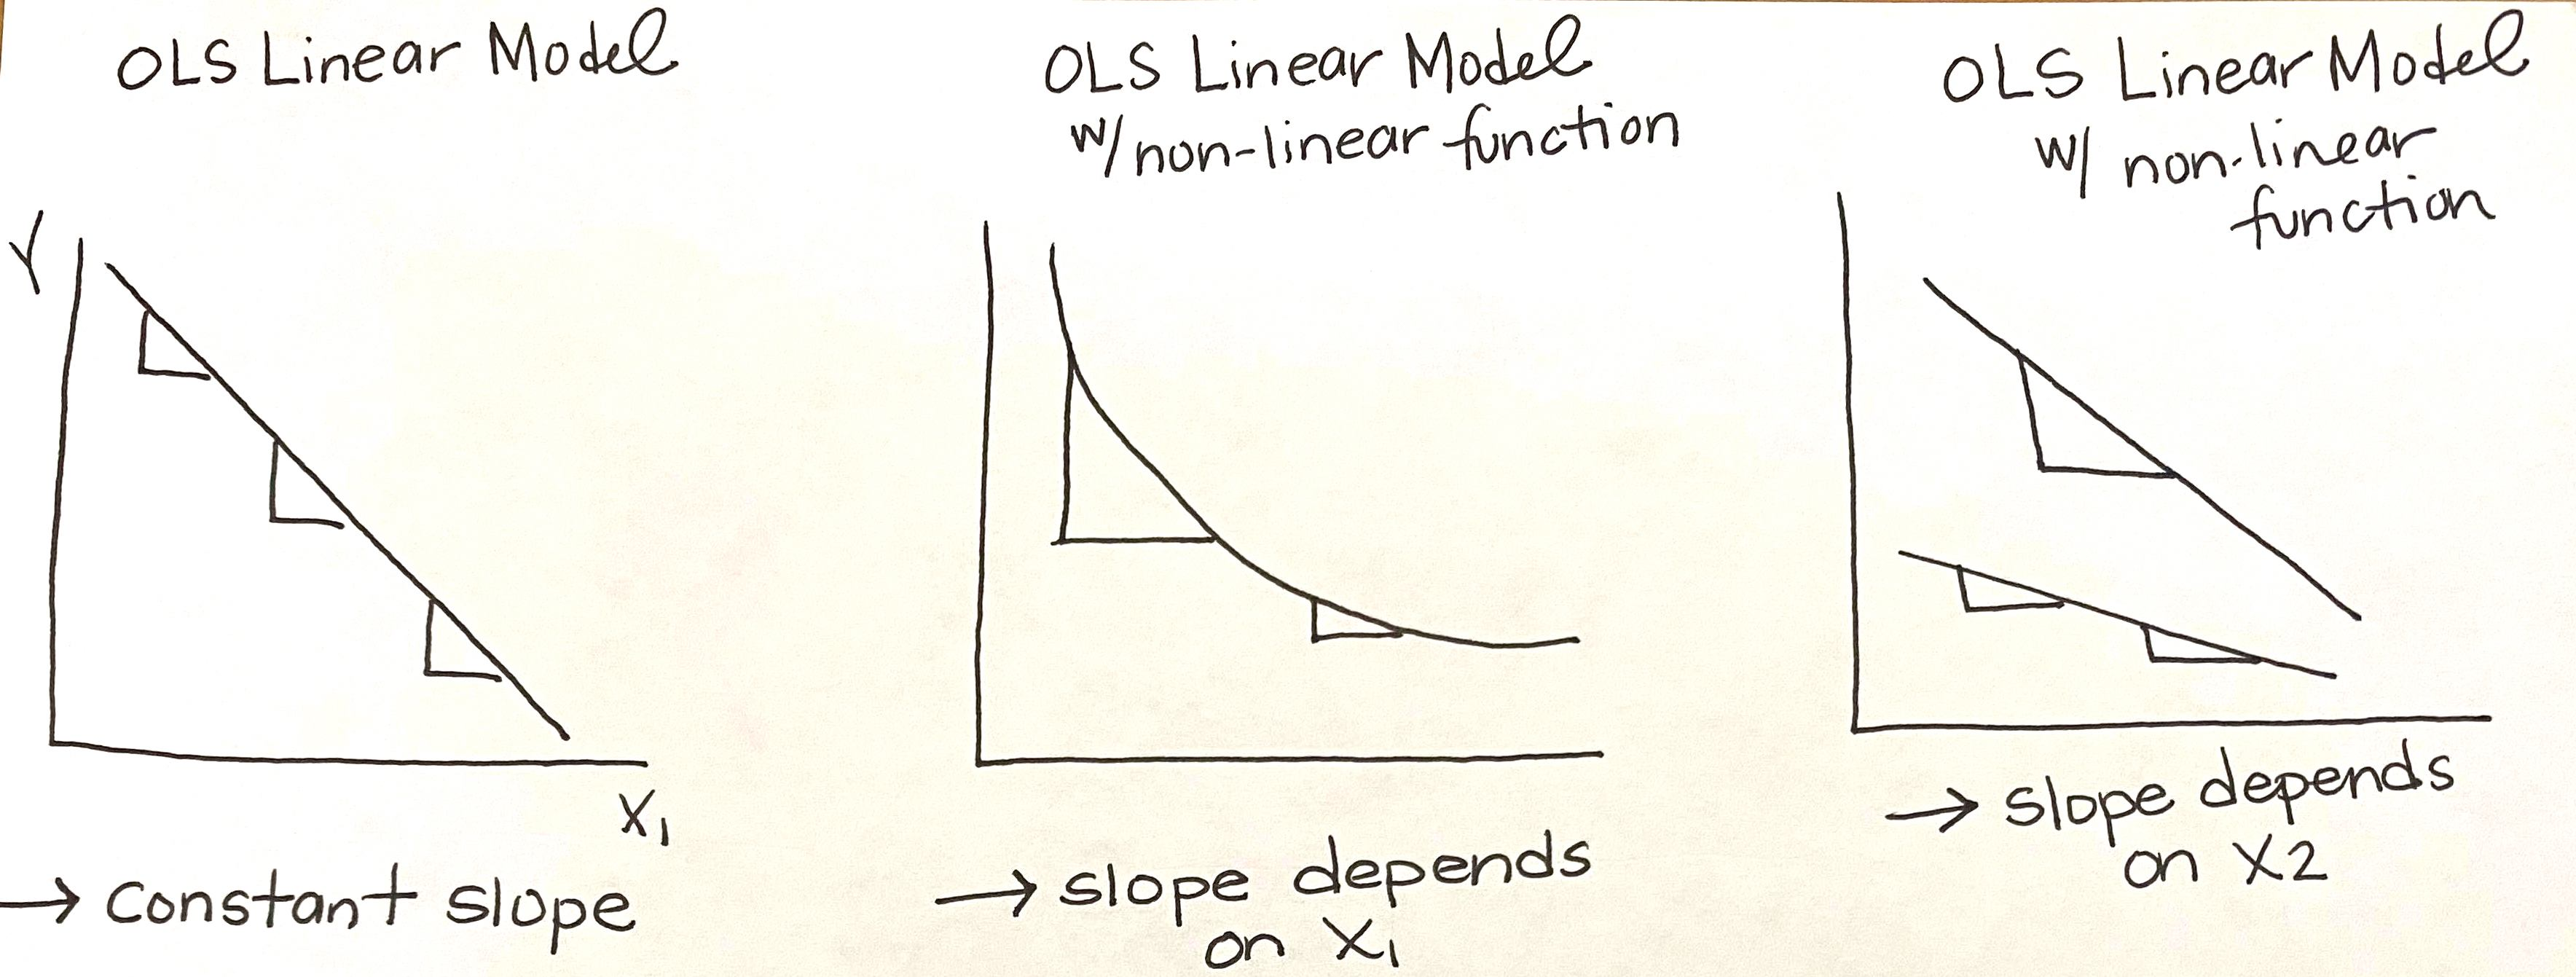
\includegraphics{slope.jpg}

\end{frame}

\begin{frame}[fragile]{Logarithms}
\protect\hypertarget{logarithms}{}

\begin{itemize}
\tightlist
\item
  Besides polynomials, another way to specify a nonlinear function using
  OLS regression is to use the natural logarithm of Y and/or X.
\item
  Logarithms allow changes in variables to be interpreted in terms of
  percentages

  \begin{itemize}
  \tightlist
  \item
    Ex: What is the effect of district income on test scores?
  \item
    A 1\% change in district income (as opposed to for instance a
    \(\$1000\) change) is associated with a \(\hat{\beta_1}\) change in
    test scores
  \end{itemize}
\item
  Regression only uses Natural Logarithm, \(ln(X)\)

  \begin{itemize}
  \tightlist
  \item
    \(ln(X)\) is the inverse of exponential function (\(e^x\))
  \item
    We dont use \(log_{10}\)
  \end{itemize}
\item
  We can use \(ln(X)\) to interpret percent changes because:

  \begin{itemize}
  \tightlist
  \item
    \(ln(X + \Delta X) - ln(X) \approx \frac{\Delta X}{X}\) when
    \(\frac{\Delta X}{X}\) is small
  \item
    In words: When the change in X is small, the difference between the
    log of X plus the change in X and the log of X is approxiately the
    percentage change in X
  \end{itemize}
\item
  Ex: \(X=100, \Delta X = 1\)

  \begin{itemize}
  \tightlist
  \item
    \(\frac{\Delta X}{X}\) = \(\frac{1}{100}\) = 0.01 (or 1\%)
  \item
    \(ln(X + \Delta X) - ln(X)\) = \(ln(100 + 1) - ln(100)\)
  \item
    plug into R console: \texttt{log(101)\ -\ log(100)} = 0.009950331
    (or 1\%)
  \end{itemize}
\end{itemize}

\end{frame}

\begin{frame}{Logarithms}
\protect\hypertarget{logarithms-1}{}

Three cases where logarithms might be used\ldots{}

\begin{enumerate}
[1)]
\tightlist
\item
  \textbf{Linear-Log Model}: When X is transformed by taking its
  logarithm but Y is not
\end{enumerate}

\begin{itemize}
\tightlist
\item
  \(Yi = \beta_0 + \beta_1\) \(ln(X_{1i}) + ui\)
\item
  We will cover this as the log transformation is on X!
\item
  Remember OLS can model nonlinear functions of the independent
  variables
\end{itemize}

\begin{enumerate}
[1)]
\setcounter{enumi}{1}
\tightlist
\item
  \textbf{Log-Linear Model}: When Y is transformed by taking its
  logarithm but X is not
\end{enumerate}

\begin{itemize}
\tightlist
\item
  \(ln(Yi) = \beta_0 + \beta_1X_{1i} + ui\)
\item
  There is substantial overlap between Log Linear Models and Logistic
  Models (non-linear model rather than non-linear function of X)
\item
  Will cover this in HED 613
\end{itemize}

\begin{enumerate}
[1)]
\setcounter{enumi}{2}
\tightlist
\item
  \textbf{Log-Log Model}: When both X and Y are transformed by taking
  their logarithm
\end{enumerate}

\begin{itemize}
\tightlist
\item
  \(ln(Yi) = \beta_0 + \beta_1\) \(ln(X_{1i}) + ui\)
\item
  Will cover this in HED 613
\end{itemize}

\end{frame}

\begin{frame}{Linear-Log Model}
\protect\hypertarget{linear-log-model}{}

\textbf{Linear-Log Model}: When X is transformed by taking its logarithm
but Y is not

\begin{itemize}
\tightlist
\item
  RQ: What is the effect of district income on student test scores?
\item
  \textbf{Pop Reg Model: \(Yi = \beta_0 + \beta_1\) \(ln(X_{1i}) + ui\)}

  \begin{itemize}
  \tightlist
  \item
    Where Y= test scores, ln(X)= log of district income
  \end{itemize}
\item
  Run in R
\item
  \textbf{OLS Prediction Line}

  \begin{itemize}
  \tightlist
  \item
    w/o estimates: \(Yi = \hat{\beta_0} + \hat{\beta_1}\) \(ln(X_{1i})\)
  \item
    w estimates: \(Yi = 557.832 + 36.42*ln(X_{1i})\)
  \end{itemize}
\item
  \textbf{Interpretation of \(\hat{\beta_1}\)}

  \begin{itemize}
  \tightlist
  \item
    General: a 1\% increase in X is associated with a
    0.01*\(\hat{\beta_1}\) change in Y
  \item
    a 1\% increase in district average income per capita is associated
    with a 0.36 point increase (0.01*36.42) in district average test
    scores.
  \end{itemize}
\item
  \textbf{Prediction}

  \begin{itemize}
  \tightlist
  \item
    Last week's example: what is the change in average student test
    scores for change in \$10k to \$11k income?
  \item
    Still the same as last week, rate of change = the difference in
    predicted test scores (\(\hat{Y}\)) of the two X values
  \item
    (\(Yi = 557.832 + 36.42*ln(11)\)) -
    (\(Yi = 557.832 + 36.42*ln(11)\))
  \item
    (645.1633) - (641.6921) = 3.4712
  \end{itemize}
\end{itemize}

\end{frame}

\begin{frame}{Conceptual Approach to Modeling Nonlinearities using
Multivariate Regression}
\protect\hypertarget{conceptual-approach-to-modeling-nonlinearities-using-multivariate-regression}{}

\textbf{When the effect of \(X_{1i}\) on Y depends on \(X_{1i}\)}

\medskip

\begin{enumerate}
\tightlist
\item
  Identify possible nonlinear relationship

  \begin{itemize}
  \tightlist
  \item
    Use theory and previous literature
  \item
    Ask yourself if the slope of the regression line relationship
    between Y and X might reasonbly depend on the value of X or another
    independent variable
  \end{itemize}
\item
  Plot the X and Y relationship; visually inspect the data!
\item
  Specify the nonlinear function that makes the most sense

  \begin{itemize}
  \tightlist
  \item
    Sometimes this is more practical than technical
  \item
    How do you want to interpret the effect of X on Y? By \% change
    (Log) or by different rates of change based on starting value of X
    (Polynomial)
  \item
    Most time our control variables are the non-linear functions, not
    our independent variable of interest
  \item
    In prediction, adding the non-linear term should increase model git
  \end{itemize}
\item
  Determine whether the nonlinear model improves upon the linear model

  \begin{itemize}
  \tightlist
  \item
    Use the t-statistic on your nonlinear coefficient!
  \end{itemize}
\item
  Replot the data using the nonlinear model; visually inspect the data
  again!
\end{enumerate}

\end{frame}

\hypertarget{linear-probability-model}{%
\section{Linear Probability Model}\label{linear-probability-model}}

\begin{frame}{Linear Probability Model}
\protect\hypertarget{linear-probability-model-1}{}

\begin{itemize}
\tightlist
\item
  Binary Variables (i.e., dummies, indicators) as dependent variables
  are very common in education research!

  \begin{itemize}
  \tightlist
  \item
    Y = Retention (0=dropped out, 1= persisted)
  \item
    Y = Graduation (0= did not graduate, 1= graduated)
  \item
    Y = Pass/Fail (0=Failed, Passed=1)
  \end{itemize}
\item
  Regression models with a binary dependent variable attempt to
  interpret the effect of X on the \emph{probability} of ``success''
  (Y=1)

  \begin{itemize}
  \tightlist
  \item
    Or in some cases the probability of ``failure''
  \end{itemize}
\item
  Most social science disciplines model binary dependent variables via
  non-linear regression models

  \begin{itemize}
  \tightlist
  \item
    logistic regression {[}will cover in HED 613{]}
  \item
    but interpretation can be difficult because of odds ratios
  \end{itemize}
\item
  Econometrics models binary dependent variables via \emph{linear
  probability model}

  \begin{itemize}
  \tightlist
  \item
    Population parameters can be estimated via OLS!
  \item
    Simple to estimate and interpret!
  \item
    Only ``tool'' that doesn't carry over? \(R^2\); but program
    evaluation is less concerned with model fit than hypothesis testing
    about the population parameter \(\beta_1\)
  \end{itemize}
\end{itemize}

\end{frame}

\begin{frame}[fragile]{Linear Probability Model, with Continuous X}
\protect\hypertarget{linear-probability-model-with-continuous-x}{}

\begin{itemize}
\tightlist
\item
  RQ: What is the effect of debt payment-to-income ratio on the
  probabibility of being denied a mortgage loan?
\item
  \textbf{Pop Reg Model: \(Yi = \beta_0 + \beta_1X_{1i} + ui\)}

  \begin{itemize}
  \tightlist
  \item
    Y = \texttt{deny}(1= mortgage loan denied, 0= mortgage loan
    approved)
  \item
    X = debt payment-to-income ratio (higher proportion = more debt,
    lower-proportion = less debt)
  \end{itemize}
\item
  Run in R
\item
  \textbf{OLS Prediction Line}

  \begin{itemize}
  \tightlist
  \item
    w/o estimates: \(Yi = \hat{\beta_0} + \hat{\beta_1}X_{1i}\)
  \item
    w estimates: \(Yi = -0.07991 + 0.604*X_{1i}\)
  \end{itemize}
\item
  \textbf{Interpretation of \(\hat{\beta_1}\)}

  \begin{itemize}
  \tightlist
  \item
    General: On average, a n-unit increase in X is associated with a
    (n-unit\(*\hat{\beta_1})*100\) percentage point change in the
    probability of Y=1
  \item
    On average, a 0.01 increase in payment-to-income ratio is associated
    with a 0.6 percentage-point increase \(((0.01*0.604)*100)\) in the
    probability of being denied a mortgage loan.
  \item
    On average, a 0.25 increase in payment-to-income ratio is associated
    with a 15 percentage-point increase \(((0.25 *0.604)*100)\) in the
    probability of being denied a mortgage loan.
  \end{itemize}
\end{itemize}

\end{frame}

\begin{frame}[fragile]{Linear Probability Model, with Categorical X}
\protect\hypertarget{linear-probability-model-with-categorical-x}{}

\begin{itemize}
\tightlist
\item
  RQ: What is the effect of an applicant's race on the probabibility of
  being denied a mortgage loan, holding debt payment-to-income ratio
  constant?
\item
  \textbf{Pop Reg Model:
  \(Yi = \beta_0 + \beta_1X_{1i} + \beta_2X_{2i} + ui\)}

  \begin{itemize}
  \tightlist
  \item
    Y = \texttt{deny}(1= mortgage loan denied, 0= mortgage loan
    approved)
  \item
    X1 = \texttt{afam}(1= African American applicant, 0= White applicant
    {[}reference group{]})
  \item
    X2 = debt payment-to-income ratio
  \end{itemize}
\item
  Run in R
\item
  \textbf{OLS Prediction Line}

  \begin{itemize}
  \tightlist
  \item
    w/o estimates:
    \(Yi = \hat{\beta_0} + \hat{\beta_1}X_{1i} + \hat{\beta_2}X_{2i}\)
  \item
    w estimates: \(Yi = -0.091 + 0.177*X_{1i} + 0.56*X_{2i}\)
  \end{itemize}
\item
  \textbf{Interpretation of \(\hat{\beta_1}\)}

  \begin{itemize}
  \tightlist
  \item
    General: On average, being in the ``non-reference group'' as opposed
    to the ``reference group'' is associated with a
    100*\(\hat{\beta_1}\) percentage point change in the probability of
    Y=1
  \item
    On average, an African-American applicant as opposed to white
    applicant is associated with a 17.7 (100*0.177) percentage point
    increase in the probability of being denied a mortgage loan, holding
    debt payment-to-income ratio constant
  \end{itemize}
\end{itemize}

\end{frame}

\end{document}
